\subsection{Grobplanung}"In der Grobplanung wurden die wichtigsten Meilensteine des Gesamtsystems und der einzelnen Disziplinen festgehalten.
Der Zeitstrahl in Abbildung \ref{fig:rahmenplanung} zeigt die chronologische Reihenfolge an. Als klar wurde, dass die Umsetzung in Verzug war, wurde die Planung angepasst.
Trotz Unstimmigkeiten des Terminplans wurde er kein zweites Mal aktualisiert, da die Zeit knapp wurde und nur wenige Punkte offen waren.

\begin{landscape}
	\begin{figure}
		\centering
		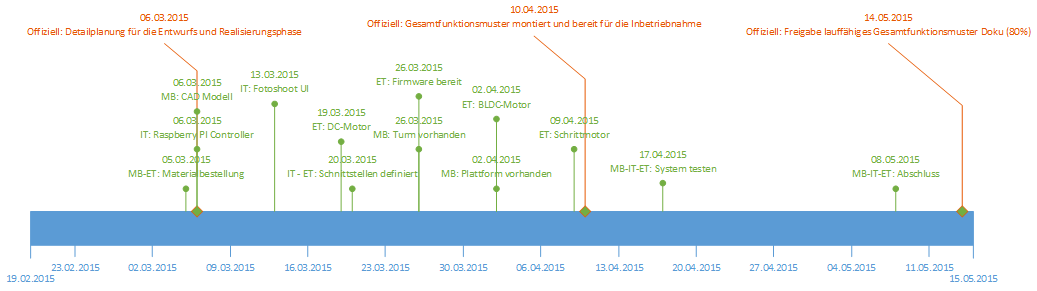
\includegraphics[width=1\linewidth]{../../fig/rahmenplanung}
		\caption{Rahmenplan}
		\label{fig:rahmenplanung}
	\end{figure}
\end{landscape}

\subsubsection{Rahmenplanung (Stand: 10.04.2015)}

Am 10.04.2015 hat sich das Team zusammengeschlossen um über die restlichen Arbeiten zu diskutieren. Darauf hin hat man sich entschlossen die restliche Planung anzupassen. Nun wurden teilweise neue Termine definiert, welche für den restlichen Verlauf bindend sind.

\begin{figure}[h!]
	\centering
	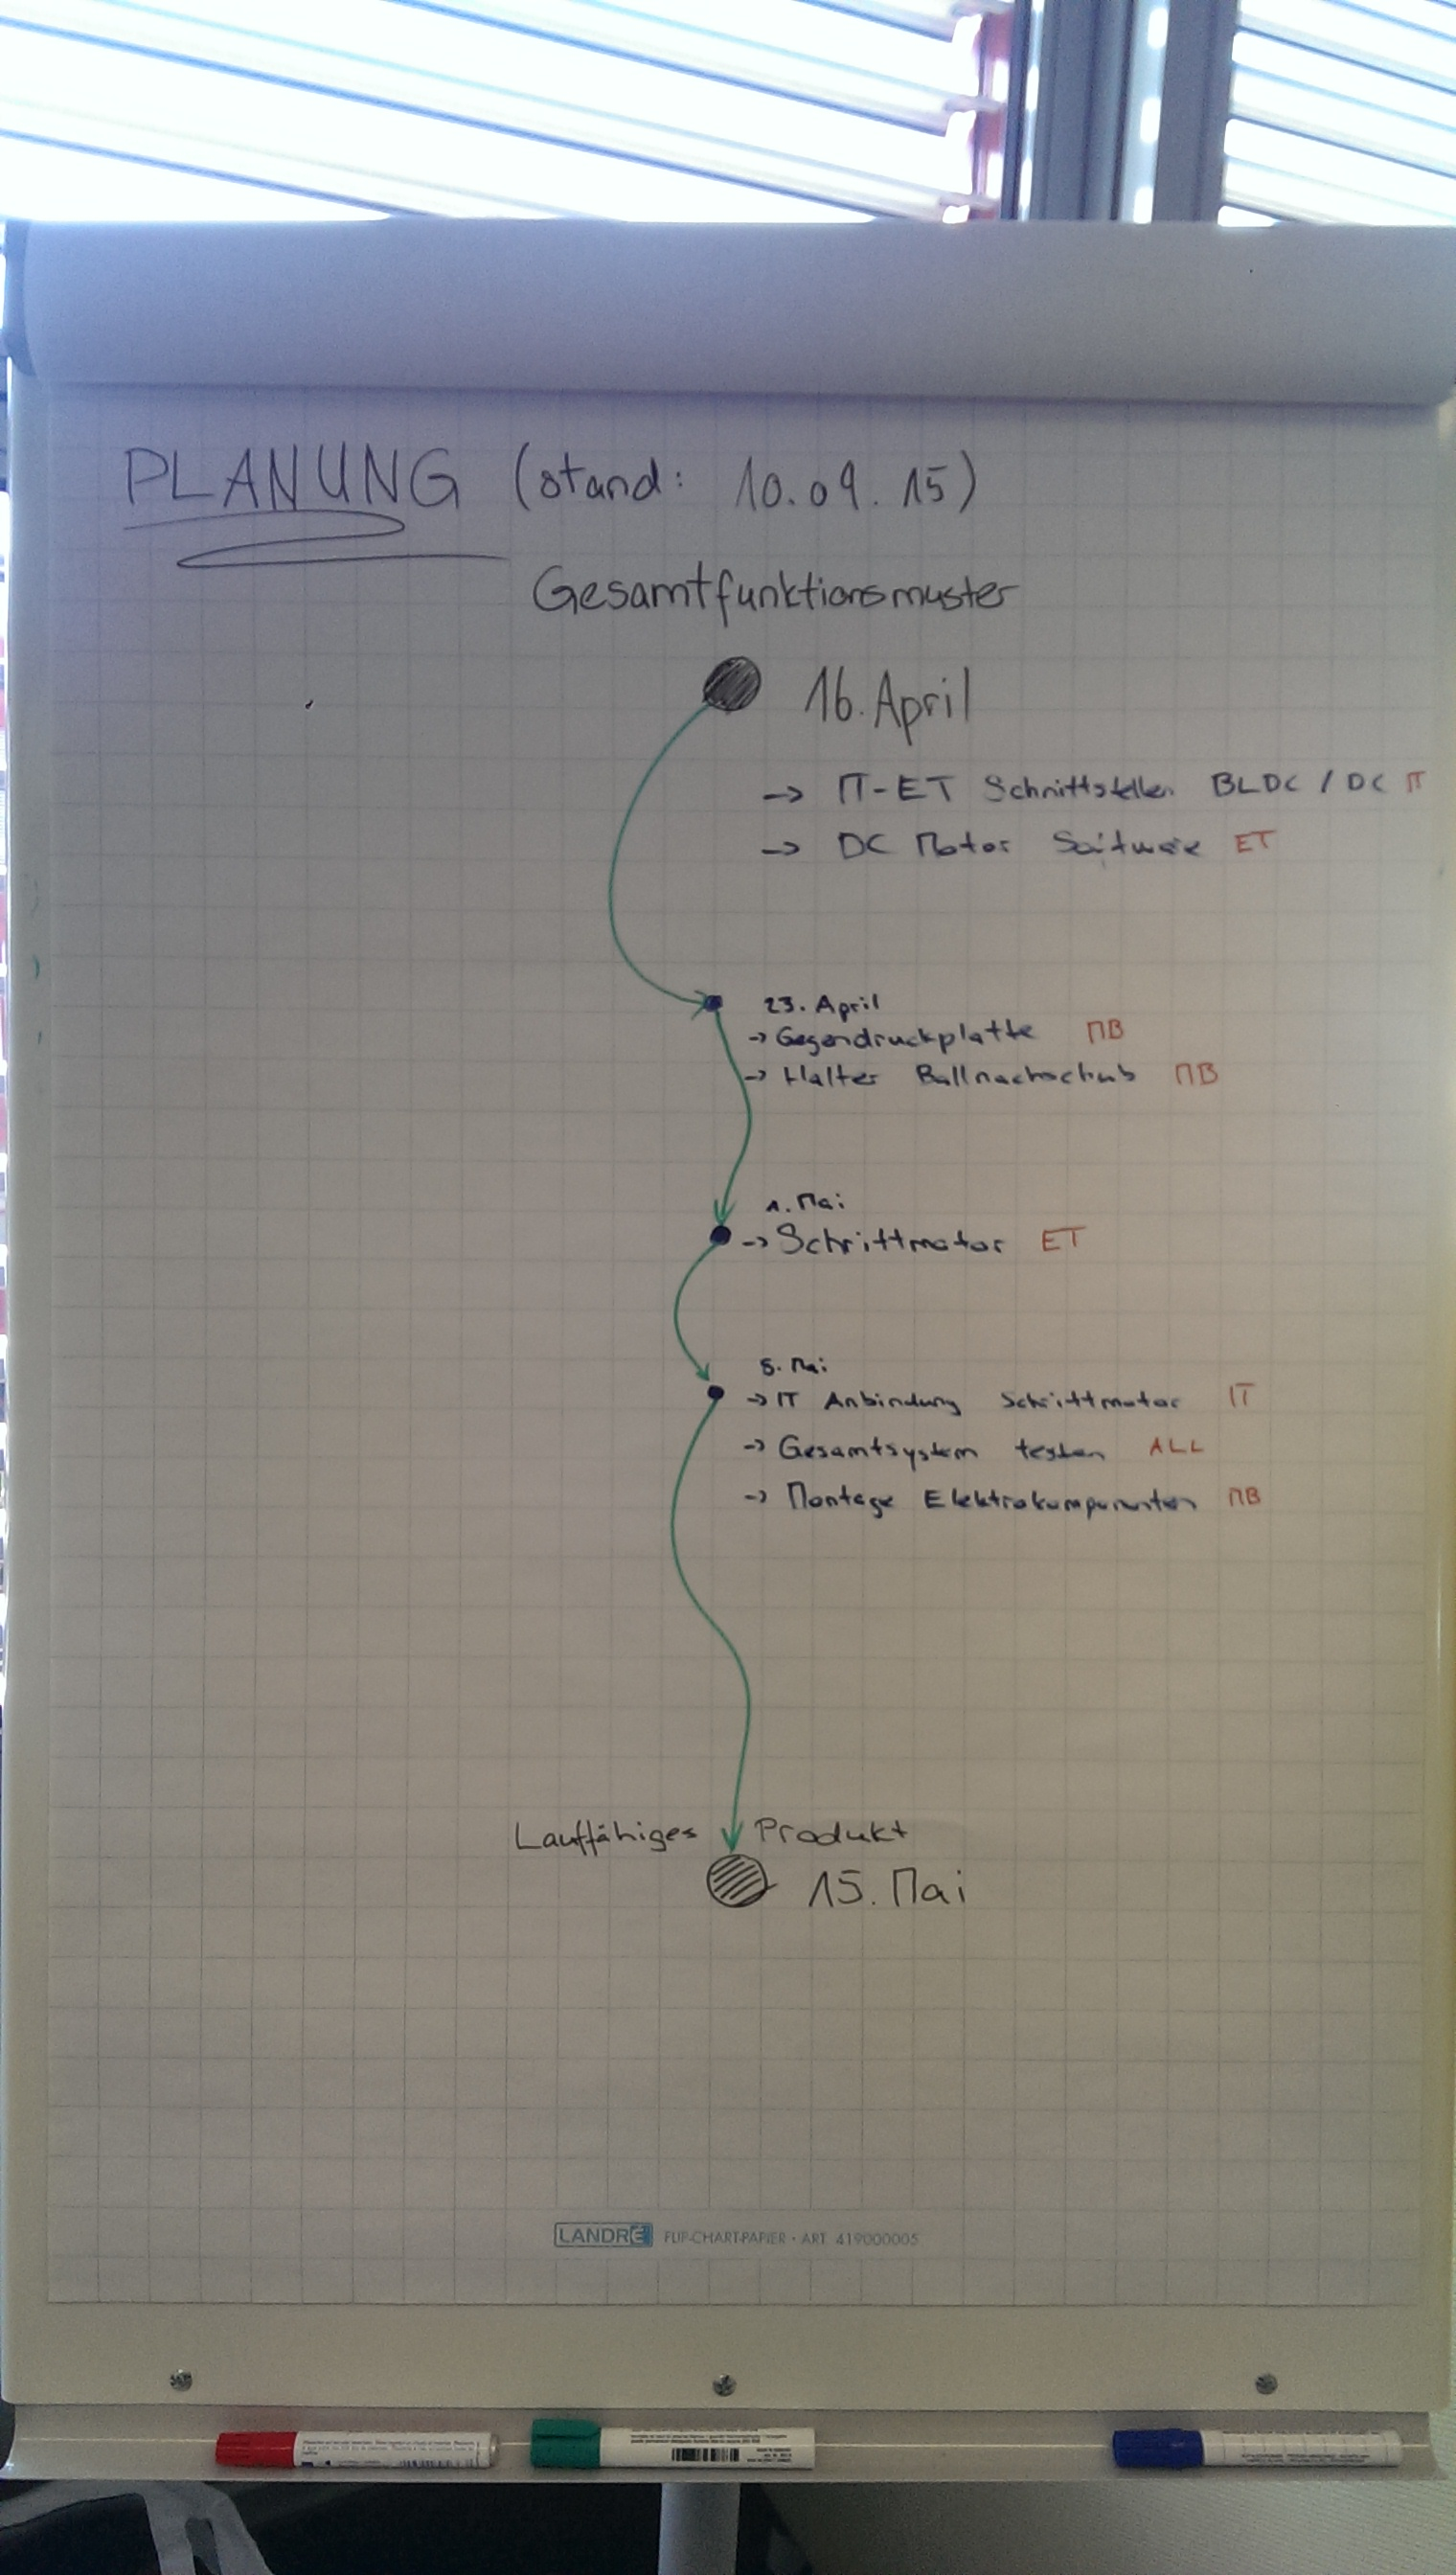
\includegraphics[width=0.6\linewidth]{../../fig/rahmenplanung-10042015}
	\caption{Rahmenlanung (Stand 10.04.2015)}
	\label{fig:rahmenplanung-10042015}
\end{figure}

\subsubsection{Fazit}

Die angepasste Rahmenplanung konnte nicht vollständig eingehalten werden. Besonders die Elektrotechnik stand unter Zeitdruck, da nur ein Projektmitglied das nötige Fachwissen besass.
Zusätzlich wurden in der Maschinentechnik diverse Bauteile verbessert und ausgetauscht. Dies verzögerte die Funktionstests um zwei Wochen.
Der Schrittmotor funktionierte ebenfalls zwei Wochen nach der angepassten Planung.
